\clearpage

\lehead[]{\sf\hspace*{-2.00cm}\textcolor{white}{\colorbox{lightblue}{\parbox[c][0.70cm][b]{1.60cm}{
\makebox[1.60cm][r]{\thechapter}\\ \makebox[1.60cm][r]{ÜBUNG}}}}\hspace{0.17cm}\textcolor{lightblue}{\chaptertitle}}
\rohead[]{\textcolor{lightblue}{\chaptertitle}\sf\hspace*{0.17cm}\textcolor{white}{\colorbox{lightblue}{\parbox[c][0.70cm][b]{1.60cm}{\thechapter\\
ÜBUNG}}}\hspace{-2.00cm}}
%\chead[]{}
\rehead[]{\textcolor{lightblue}{AvHG, Inf, My}}
\lohead[]{\textcolor{lightblue}{AvHG, Inf, My}}

\section{Tastaturereignisse -- Übungen}

\subsection{Aufgabe 1: Leseübung}

Hier siehst du ein Beispielprogramm, das Tastatureingaben verarbeitet.
Kannst du die Bedeutung der hervorgehobenen Methoden und Schlüsselwörter
erklären?

\begin{lstlisting}
æimport java.awt.Color;
import java.awt.EventQueue;
import java.awt.Graphics;
import java.awt.event.KeyEvent;
import java.awt.event.KeyListener;
import hilfe.*;

public class Zeichnen extends HJFrame æimplements KeyListeneræ {
    private static final final int WIDTH = 500;
    private static final int HEIGHT = 500;
    private static final Color BACKGROUND = Color.WHITE;
    private static final Color FOREGROUND = Color.BLACK;
    private boolean bKreisZeichnen = false;

    public Zeichnen(final String title) {
        super(WIDTH, HEIGHT, BACKGROUND, FOREGROUND, title);
        æaddKeyListener(this);æ
    }

    @Override
    public void myPaint(Graphics g) {
        if (bKreisZeichnen) {
            g.drawString("Wenn du 'L' drückst, lösche ich den Kreis.", 20, 50);
            g.drawOval(50,100, 100,100);
        } else {
            g.drawString("Wenn du 'M' drückst, male ich einen Kreis.", 20, 50);
        }
    }

æ    @Override
    public void keyPressed(KeyEvent e) { 
        int c = e.getKeyCode();
        switch (c) {
            case KeyEvent.VK_M:         æ// Taste 'M' (egal ob groß oder klein)
æ                bKreisZeichnen = true;
                repaint();              æ// Bildschirm neu malen
æ                break;
            case KeyEvent.VK_L:         æ// Taste 'L'
æ                bKreisZeichnen = false;
                repaint();              æ// Bildschirm neu malen
æ        }
    }

    @Override
    public void keyReleased(KeyEvent e) {}

    @Override
    public void keyTyped(KeyEvent e) {}æ

    public static void main(final String[] args) {
        EventQueue.invokeLater(new Runnable() {
            public void run() {
                try {
                    Zeichnen anwendung = new Zeichnen("Zeichnen");
                } catch (Exception e) {
                    e.printStackTrace();
                }
            }
        });
    }
}
\end{lstlisting}


\subsection{Aufgabe 2: Game of Life}

Das „Game of Life“ soll mit Hilfe von Tastaturbefehlen gesteuert werden können.

\begin{compactenum}[a)]
\item Neustart

Wenn der Benutzer ein kleines oder großes ’N’ drückt, soll das zweidimensionale
boolesche Array mit neuen Zufallswerten versehen werden, so dass die Simulation
quasi neu startet.

\item Anhalten und weiter machen

Der Ablauf der Simulation kann angehalten und anschließend wieder fortgesetzt
werden. Wenn der Benutzer ein kleines oder großes ’A’ drückt, soll der Timer
ausgeschaltet werden, damit das Bild eingefroren wird. Wenn der Benutzer ein
kleines oder großes ’W’ drückt wird der Timer wieder gestartet.

\item Geschwindigkeit variieren: langsam, mittel oder schnell

Der Ablauf der Simulation kann in verschiedenen Geschwindigkeiten geschehen.
Dazu gibt es drei Stufen: ’l’ für langsam, ’m’ für mittel und ’s’ für schnell.
Zu Beginn startet die Simulation mit einer mittleren Geschwindigkeit. Wenn der
Benutzer eine der drei Tasten zur Änderung der Geschwindigkeit drückt, wird der
Timer kurz ausgeschaltet und anschließend erneut gestartet mit einer
Geschwindigkeit, die dem gewünschten Level entspricht.

Achte darauf, dass die Simulation nach einer Pause (die in Teil b programmiert
wurde) mit der Geschwindigkeit des zuletzt gewählten Levels weiter läuft.
\end{compactenum} 


\subsection{Aufgabe 3: Stoppuhr}

Vor einiger Zeit haben wir eine Klasse \myClass{Uhr} programmiert. Leite eine
Unterklasse von der Klasse Uhr ab, und erweitere sie zur Stoppuhr. Die Stoppuhr
soll mit dem Messen der Zeit beginnen, wenn die Taste ’S’ gedrückt wird (für
\glqq Start\grqq ). Wenn die Taste ‚E’ gedrückt wird (für \glqq Ende\grqq ),
soll die Zeitmessung beendet werden. Das Drücken auf ’R’ (für \glqq Reset\grqq )
setzt die Uhrzeit auf 00:00 zurück.

Die ursprüngliche Klasse \myClass{Uhr} soll unverändert erhalten bleiben, damit
man sie weiterhin benutzen kann. Die Klasse \myClass{Ziffer} darf jedoch um eine
Methode zum Zurückstellen der Ziffer auf Null ergänzt werden.


\subsection{Aufgabe 4: Dartspiel}

Ein Pfeil wird auf eine Dartscheibe abgeschossen. Der Benutzer muss versuchen,
die Mitte der Zielscheibe zu treffen.

\begin{center}
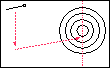
\includegraphics[width=0.2\textwidth]{./inf/SEKII/21_Java_Tastaturereignisse/Dartspiel.png}
\end{center}

Auf dem Bildschirm werden eine fest positionierte Zielscheibe und ein Pfeil
dargestellt. Der Pfeil ist leicht nach oben geneigt, damit das Spiel nicht zu
einfach wird. Das Spiel beginnt, sobald der Benutzer die Taste ’N’ drückt (für
„Neues Spiel“). Der Pfeil fällt senkrecht nach unten. Der Benutzer muss den
Pfeil zum richtigen Zeitpunkt durch Drücken der Taste ’S’ (für „Schuss“)
abschießen. Der Pfeil fliegt dann in der eingeschlagenen Richtung auf die
Scheibe zu. Er landet, sobald er die imaginäre Mittellinie der Scheibe erreicht
hat. Drückt man die Taste ’N’ erneut, so beginnt ein neues Spiel. Der Pfeil
wird wieder an die Anfangsposition gesetzt und fällt sofort senkrecht nach unten.

Tipps: Für die Zielscheibe braucht man keine eigene Klasse programmieren. Sie
kann in der \lstinline|myPaint()|-Methode des Anwendungsfensters gezeichnet
werden. Eine eigene Klasse muss nur für den Pfeil geschrieben werden. Überlege
dir zunächst, welche verschiedenen Zustände ein Pfeil besitzt. Zeichne dazu ein
UML-Zustandsdiagramm. Beachte auch, dass der Pfeil die x-Position der
Scheiben-Mitte kennen muss, damit er weiß, wann er sein Ziel erreicht hat. Die
Mittellinie und die Geschwindigkeit des Pfeils in x-Richtung sollten so
aufeinander abgestimmt werden, dass der Pfeil die Mittellinie genau trifft.


\subsection{Aufgabe 5: Autorennen}

Ein Auto muss in möglichst kurzer Zeit um eine Reihe von Hindernissen herum
navigiert werden. Es gibt eine Taste zum Erhöhen der Geschwindigkeit und eine
Taste zum Abbremsen. Zwei weitere Tasten ermöglichen es, das Auto während der
Fahrt nach links oder rechts zu steuern (es reicht, einfach die „x-Position“ zu
verschieben). Wenn das Auto gegen ein Hindernis prallt, hat der Benutzer das
Spiel verloren. Das Programm misst die Zeit des Spielers und zeigt sie am Ende
an. Die Zeitmessung kann mit der statischen Methode
\lstinline|currentTimeMillis()| aus der Klasse \myClass{System} erfolgen:

\begin{lstlisting}
long t1, t2;
t1 = System.currentTimeMillis();
æ... hier passiert was auch immer du zeitlich messen möchtest
æt2 = System.currentTimeMillis();
System.out.println("Es sind " + (double) (t2 - t1) / 1000.0 + "Sekunden vergangen");
\end{lstlisting}

Es empfiehlt sich, das Rennen aus der Vogelperspektive zu zeichnen (siehe Skizze).

\begin{center}
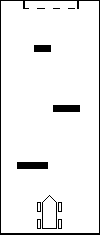
\includegraphics[width=0.2\textwidth]{./inf/SEKII/21_Java_Tastaturereignisse/Autorennen.png}
\end{center}

Mögliche Erweiterung:

Zwei Spieler spielen gleichzeitig gegeneinander. Jeder Spieler hat sein eigenes
Auto, das er mit einer eigenen Tastenkombination steuert.


\subsection{Aufgabe 6: Streifen}

\begin{compactenum}[a)]
\item Programmiere eine Klasse \myClass{Streifen}. Im Konstruktor der Klasse
\myClass{Streifen} soll zunächst nur die y-Position eines Streifens als
Parameter übergeben werden. Die x-Position wird fest auf 100 gesetzt und die
Breite und die Höhe werden jeweils auf 30 Pixel eingestellt. Alle Variablen der
Klasse sollen vor dem Zugriff von außen versteckt sein. Die Klasse
\myClass{Streifen} enthält eine Methode \lstinline|zeichnen()|, die den Streifen
als gefülltes rotes Rechteck mit den eingestellten Koordinaten malt.

Erzeuge im Anwendungsfenster in einer Schleife ein Array von zehn Streifen. Der
erste Streifen soll die y-Position 40 besitzen. Der zweite Streifen besitzt die
y-Position 80, der dritte die y-Position 120, der vierte die y-Position 160,
und so weiter.

\item Die Breite der Streifen soll durch Tastendrücke verstellt werden können.
Dazu erhält jeder Streifen in alphabetischer Reihenfolge jeweils einen
Buchstaben in Klein- und in Großschreibung zugewiesen. Der erste Streifen
erhält ’a’ und ’A’, der zweite ’b’ und ’B’, und so weiter. Der letzte Streifen
wird durch ’j’ und ’J’ gesteuert.

Wenn man den Buchstaben als Großbuchstaben drückt (z.B. ’C’), soll die Breite
des entsprechenden Streifens um zehn Pixel wachsen. Wenn man den Buchstaben als
Kleinbuchstaben drückt (z.B. ’c’), soll die Breite um zehn Pixel verringert
werden.

Sie soll allerdings nie unter zehn Pixel fallen. Wenn man bei einer Breite von
zehn Pixeln den Kleinbuchstaben drückt, wird die Eingabe ignoriert. Beachte,
dass das Anwendungsfenster nach jedem Tastendruck neu gezeichnet werden muss.
Erweitere den Konstruktor der Klasse \myClass{Streifen} so, wie es für die
Lösung dieser Aufgabe erforderlich ist.
\end{compactenum}

\begin{center}
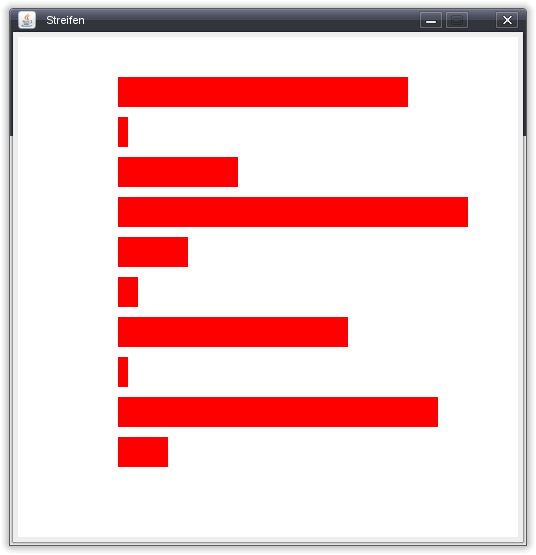
\includegraphics[width=0.6\textwidth]{./inf/SEKII/21_Java_Tastaturereignisse/Streifen.png}
\end{center}
